\documentclass[journal]{IEEEtran}

\usepackage{cite}
\usepackage{hyperref}
\usepackage{graphicx}

\usepackage{amsmath}
\interdisplaylinepenalty=2500

\usepackage{listings}
\lstset{basicstyle=\ttfamily\small, breaklines=true}

% correct bad hyphenation here
\hyphenation{op-tical net-works semi-conduc-tor}

\usepackage{xcolor}

\begin{document}

\title{Using Fuzzy Logic for extracting department from email content}
\author{Peter Heemskerk, Stefan Schenk, Jim Kamans\\11988797, 11881798, 10302905}

% The paper headers
\markboth{Using Fuzzy Logic for extracting department from email content}{}

\maketitle

\begin{abstract}
Large organizations often struggle to deliver emails or form emails to their corresponding departments if they are not directly addressed to a department or employee. In this project a Fuzzy Logic approach is proposed for automatically determining the correct department. 

[dit stukje redigeren op basis van laatste resultaten:]
First results are promising and results in correct department determination  of xx perc. The set-up of the systems is also flexible to add more flexibility to determine departments not only on content based features but also based on more general feature (as " emotion" ) of the email content. 

\end{abstract}

\section{Introduction}
\IEEEPARstart{M}{any} large organizations suffer from their own complexity. If an external party seeks contact with a specific person in an organization, this usually works fine, but if a party seeks contact about a subject (without knowing whom to talk to), it usually takes more time before the party gets a good answer, simply because it is not clear what the right department is which should reply on such a message. At this moment emailing is the main way of communication to businesses, 120 billion emails a year are sent which figure includes a large portion of spam mail \cite{email_statistics}.\\

%\subsection{Problem}

This project aims to solve this issue of low customer service in a complex organization. We present software based on fuzzy logic which aims to bring a message of an external party to the correct internal department purely based on the content of the message.

This project aims to demonstrate that Fuzzy Logic has advantages toward other methods. Why would that be? Firstly, fuzzy logic deals well with incomplete or difficult to interpret data. Since there is a variety of email messages, short and long, specific and vague, fuzzy logic better deals with these different sources. Secondly, fuzzy logic uses linguistic terms. With this we can include expert knowledge into the system which is relatively easy to interpret.

%\subsection{Objectives}

The experiment has the goal to determine the correct department from email content. Based on the cleaned word lists a feature vector will be determined for each email. For department determination content specific features are used. These features are used as inputs in the fuzzy logic system to finally determine as output the correct department. Our results will be compared to the given labels of the data-set.\\

\section{Literature reviews}

Fuzzy Logic has been used earlier for email classification. Ferolin \cite{phishing}
has used fuzzy logic to implement a anti-phishing tool using content- and non-content email parameters. A RIPPER Classification Algorithm is used to learn relations of different phishing features, which translate into Fuzzy Logic rules. Santhi et al \cite{spam} determined the degree of dangerousness of spam email with a different method. A Fuzzy Logic system is used to categorize words that are spam in the degree to which these words are considered dangerous. The words are labeled to five linguistic variables which are input for the fuzzy logic algorithm. Ferolin \cite{ranking} introduced a fuzzy logic based ranking function for efficient Information Retrieval. A fuzzy approach was used to rank words based on term-weighting schemes such as term frequency, inverse document frequency and normalization. The term frequency and inverse document frequency and normalization of the query and document are fed to their Fuzzy Logic Controller, whose outputs are fed to the main Fuzzy Logic Controller, which outputs a relevance score. None of these has utilized fuzzy logic for determining departments.

Douglass \cite{ranking} developed an email priority setting learning system for G-mail based on social, content, search label features. These features are use in a statistical model which is parametrized for each user (recipient) separately. This research does not present a solution for situations in larger organizations where there is no information about the individual recipient.

\section{Approach}
For our department determination we follow the procedures proposed by Ferolin for Information Retrieval. The following approach is followed. After data-pre-processing the email words are ranked, resulting in a feature score per email. Ranking is done against a word dataset as details in data-preparation. Then fuzzy logic is applied to classify the email to the correct department.

\subsection{Data}

A private dataset from ``Gemeente Amsterdam'' is used, containing 3589 emails with complaints from citizens.
This dataset is a csv-file where each email has a correct department label, a description of the complaint, a description of contact with an employee and a proposed solution.
An example:
\begin{lstlisting}
Parkeren;Vrijdag voor een ...;Ja, contact
gezocht ...;De 23 euro ...
\end{lstlisting}

\subsection{Data preprocessing}
The data needs to be cleaned and filtered.

\begin{enumerate}
    \item Cleaning

    As an email body is read from the file system as plain text, individual terms are stored as individual values (``tokenized''). After that, capital characters are converted to lower case, punctuation and special characters are removed, stop-words are removed and the words are reduced to their base root form (``stemmed'').

    \item Filtering

    The next operation will perform an intersection between the words and a list of predefined relevant words. Words which are not in these relevant word lists are removed. As the last filtering step, the words are counted, and a corpus is created.
    
    [Stefan, klopt bovenstaand Filtering nog steeds ? ]

\end{enumerate}

\subsection{Feature word-list preparation}

[stefan checken of deze paragraaf klopt. ]

In order to create a feature score for each email (refer to section Ranking), feature word-lists are necessary. Other predefined sets of words within the set of relevant words share the same characteristics. For example a set $T \subseteq R$ exists where $T$
is the set of technical words, and $R$ is the set of relevant words from before. Feature list of technical words: $T = [t_1, t_2, \dots, t_n]$.
Other feature lists contain other themed words: $U$, $V$, $W$.\\

Feature word-lists are created using the term frequency / inverse document frequency (tf-idf) method. [ hier nog referentie toevoegen, Jim ?] From the corpus of training emails with the specific department label the following values are calculated for each term. 
\begin{center}
    $tdifd(t) = tf(t) * idf(t)$,
\end{center}
where tf(t) equals the count of terms t, and idf give a ranking of the importance of the word in the whole corpus: 
\begin{center}
    $idf(t, D) = log\dfrac{N(D)}{n_t(D)}$, 
\end{center}
where $N(D)$ is the total number of documents and $n_t(D)$ equals the number of documents containing the specific term. 
Selecting those terms with a $tdifd > treshold$, the feature-word lists are created, with signal words for the specific department.

\subsection{Ranking}

For this experiment the content type of feature determines the subject of the email.

For every word in the email that is present in $T$, a score is calculated that takes the count of that word into account in relation to the total number of relevant words in the email. This calculation is made for all feature lists ($T$, $U$, $V$, $W$), for every word in the email. 

So for each email a feature vector is determined, containing the score between 0 and 1 against the features, as defined by the feature word-lists. 

\subsection{Classification with Fuzzy Logic}

For determining the output variable department four content input variables are defined, corresponding with the content features. Refer to table \ref{table:1}. Since these are mostly chosen as a default, also now for each of the input variables 3 triangular membership functions (ms) are chosen to represent a low, medium or high value. For the output, a variable is created for each of the four departments, each variable containing 3 triangular membership functions low, medium, high.

We have set a rule base for determining departments based on the content input variables and a rule base for determining priority based on the general input variables. An overview of Rules you can find in attachment. [Jim to create] \\

\begin{figure}
	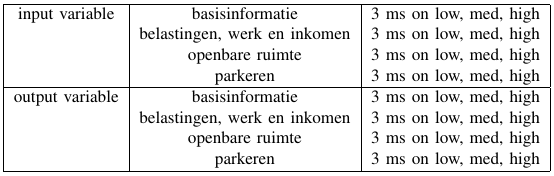
\includegraphics[scale=0.5]{res/inputs_outputs_FLS.png}
	\caption{Input and Output variables in Fuzzy Logic System}
	\label{table:1}
\end{figure}

\begin{center}
\begin{tabular}{ |c|c|c| }
 \hline
 input variable & basisinformatie   & 3 ms on low, med, high    \\
                & belastingen, werk en inkomen & 3 ms on low, med, high \\
                & openbare ruimte   & 3 ms on low, med, high    \\
                & parkeren          & 3 ms on low, med, high    \\
 output variable& basisinformatie   & 3 ms on low, med, high    \\
                & belastingen, werk en inkomen & 3 ms on low, med, high \\
                & openbare ruimte   & 3 ms on low, med, high    \\
                & parkeren          & 3 ms on low, med, high    \\
\hline
\end{tabular}
\label{table:1}
Input and Output variables in Fuzzy Logic System
\end{center}

\colorbox{yellow}{figure with rules - JIM}

\subsection{Training and validation}

For training and validating the data set is divided in a training set and validation set, with a factor 0.5 [Stefan to confirm overigens vind Muriel dit te laag, zou liever een factor 0.7 zien, kan dit nog makkelijk ?]. 

The training set of emails is used for the creation of the feature word-lists using tf/idf. The setting of the Fuzzy Logic rule base is done based on the expert vision of one of the team-members. 

The validation set including the department label is used for validation. 

\subsection{Implementation}

For cooperation purposes we used Github \footnote{\url{https://github.com/Menziess/Fuzzy-Logic-Email-Classification}} (for source control) and Trello \footnote{\url{https://trello.com/fuzzylogicemailclassification}} (as scrum projectmanagement tool)

We used Python3 as programming language and Jupyter Notebook as development
environment. The code is enlisted in Attachment [ref]. For data-preprocessing Pythons NLTK module \footnote{\url{http://www.nltk.org/}} is used. For classification a new algorithm has been developed. The fuzzy logic system itself is based on the Fuzzy Logic LAB \footnote{\url{https://blackboard.uva.nl/webapps/blackboard/execute/content/file?cmd=view&content_id=_6947429_1&course_id=_212301_1&framesetWrapped=true}}, amended for using more than one output, a centroid defuzzifier and some more flexibility and error handling in management of fuzzy logic rules.

\section{Experiment}

\subsection{Results}

The automatic process of feature word-list creation, data-preprocessing, ranking and classification with fuzzy logic has been implemented. The process is tested and works.

Validating the calculated departments with known labels has resulted in a xx percent correctness. [ Stefan / Jim]

\subsection{Discussion}

In this project a feature vector was used which corresponds to the departments already. Therefore the inclusion of Fuzzy Logic may seem a bit unnecessary. Inclusion of a feature vector has an important advantage that also non-content features (like: "press sensitive") can be extracted which may result in determining a different department. 

[Opmerking van Muriel: vooral veel aandacht aan discussie, keuzes die gemaakt zijn geven. Dus deze paragraaf nu aandacht aan geven allemaal: 
- be critical about why our process does not work
- couild we decide whether the model or the data is the bottleneck ? 
- be critical about our fuzzy logic systems setting]


\section{Acknowledgment}

This work is done as part of the autumn 2017 bachelor course Fundamentals of Fuzzy Logic by A. Bilgin (and  M. Hol and V. Dankers) within the study Artificial Intelligence at University of Amsterdam.

\begin{thebibliography}{9}
\bibitem{email_statistics}
    The Radicati Group, inc.(2015),
    \textit{
        \href{https://github.com/Menziess/Fuzzy-Logic-Email-Classification/raw/master/report/res/a_new_fuzzy_logic_based_ranking_function_for_efficient_information_retrieval_system.pdf}{Email Statistics Report, 2015-2019},
    }.

\bibitem{spam}
    G.Santhi, S. Maria Wenish, Dr. P. Sengutuvan (2013),
    \textit{
        \href{https://github.com/Menziess/Fuzzy-Logic-Email-Classification/raw/master/report/res/a_content_based_classification_of_spam_mails_with_fuzzy_word_ranking.pdf}{A Content Based Classification of Spam Mails with Fuzzy Word Ranking},
    }
    Department of Information Science and Technology,
    Issue 3.

\bibitem{phishing}
    Rosana J. Ferolin, (2010 - approx.)
    \textit{
        \href{https://github.com/Menziess/Fuzzy-Logic-Email-Classification/raw/master/report/res/a_proactive_anti-phishing_tool_using_fuzzy_logic_and_ripper_data_mining_classification_algorithm.pdf}{A Proactive Anti-Phishing Tool Using Fuzzy Logic and RIPPER Data Mining Classification Algorithm},
    }
    Department of Computer Engineering University of San Carlos.

\bibitem{ranking}
    Rosana J. Ferolin, (2014)
    \textit{
        \href{https://github.com/Menziess/Fuzzy-Logic-Email-Classification/raw/master/report/res/a_new_fuzzy_logic_based_ranking_function_for_efficient_information_retrieval_system.pdf}{A new fuzzy logic based ranking function for efficient Information Retrieval system},
    }
    Department of Electrical Engineering Dayalbagh Educational Institute.

\bibitem{priority}
    Douglas Aberdeen, (2010 approx.)
    \textit{
        \href{[nog toevoegen}{The Learning behind Gmail Priority Inbox}
    }

\end{thebibliography}

\end{document}


